Your literature review goes here. Here we show a little mathematics and figure from \cite{baek2019}.

\begin{align} 
    {W_{i + 1}} &= {W_i} + \eta ({\left\langle {{v_i}{h_i}} \right\rangle _{P(h\left| v \right.)}} - {\left\langle {{v_i}{h_i}} \right\rangle _{{\text{recon}}}})\label{eq:b1}\\ 
    {b_{i + 1}} &= {b_i} + \eta ({\left\langle {{v_i}} \right\rangle _{P(h\left| v \right.)}} - {\left\langle {{v_i}} \right\rangle _{{\text{recon}}}})\label{eq:b2}\\ 
    {a_{i + 1}} &= {a_i} + \eta ({\left\langle {{h_i}} \right\rangle _{P(h\left| v \right.)}} - {\left\langle {{h_i}} \right\rangle _{{\text{recon}}}})\label{eq:b3} 
\end{align} 

Note that the equations are labeled so that they can be referenced in the text.  For example, \ref{eq:b3} refers to the 3rd equation above.  Figures are also referencable, like this: \ref{fig:example}.

\begin{figure}
    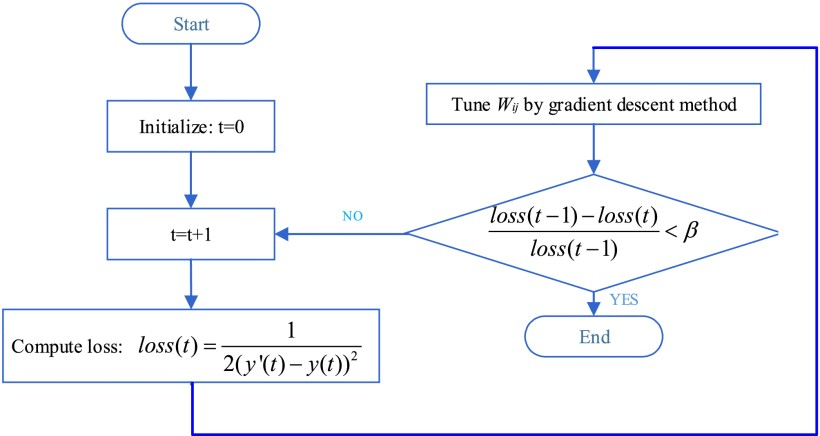
\includegraphics[width=0.8\textwidth]{baek4-2880511-large.jpg}
    \caption{Back-propagated fine-tuning process. \cite{baek2019}}
    \label{fig:example}
\end{figure}